\begin{frame}{北海道は読みにくい：\\暦で減らせる誤差は 17 \%}{考察}
  \begin{columns}[T]
    \begin{column}{0.34\textwidth}
      \bignum{17}{\%}{北海道：時期を知って減る\\落下位置の誤差}
      \vskip 3mm
      \midnum[wcOrange]{45}{\%}{和歌山（分散では 31 対 70 \%）}
    \end{column}
    \begin{column}{0.64\textwidth}
      {\centering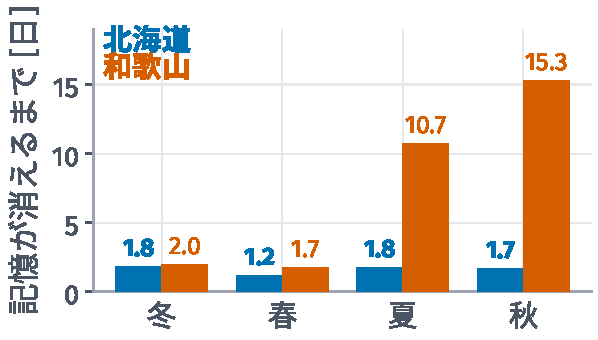
\includegraphics[width=0.86\linewidth,height=84pt,keepaspectratio]{S_decorrelation_200.pdf}\par}
      \vskip 0.5mm
      \sub{和歌山は夏・秋に 10--15 日、北海道は\kw{2 日}で入れ替わる。\\流れが止まらないので、記憶も伸びない。}
    \end{column}
  \end{columns}
  \srcline{200 hPa。風の偏差の自己相関が 1/e を切るまでの時間、2016--2025}
\end{frame}
